\ifx\wholebook\relax \else

\documentclass[b5paper]{ctexart}
\usepackage[nomarginpar
  %, margin=.5in
]{geometry}

\addtolength{\oddsidemargin}{-0.05in}
\addtolength{\evensidemargin}{-0.05in}
\addtolength{\textwidth}{0.1in}

\usepackage[cn]{../prelude}

\setcounter{page}{1}

\begin{document}

\title{零}

\author{刘新宇
\thanks{{\bfseries 刘新宇} \newline
  Email: liuxinyu99@hotmail.com \newline}
  }

\maketitle
\fi

\markboth{零}{数的旅程}

\ifx\wholebook\relax
\chapter{零}
\fi

\epigraph{因此“有”与“无”的真理,就是两者的统一。}{黑格尔《小逻辑》}

尽管数有超过5000年的历史,零却只有1200年的历史,是个“新生事物”。零诞生于印度,经由阿拉伯人引入欧洲。但它仅仅具有“占位符”的特殊身份,和1、2、3……其它数比起来是个“二等公民”,甚至面临被“开除数籍”的风险。

\section{质疑与否定}
零一出生就代表“无”、“没有”。印度人给它起名叫sunya,意为“空位”。所以2025中的0表示\underdot{没有}百。在西方,“无\footnote{对应的英文是void,表示虚空。}”在文化传统、宗教哲学上是负面否定的。它往往和黑暗、虚空、死亡等意象关联。而1代表\underdot{有}一个,2代表\underdot{有}两个……人们不说0,而说\underdot{没有},表示对\underdot{有}、\underdot{生存}、\underdot{实在}的否定。莎士比亚《王子复仇记》中的名句“To be or not to be, that is the question.”中译为“生存还是死亡?”人们说3只羊跑了1只羊,还有两只羊;如果再跑了两只羊,人们说没有羊,而不说有0只羊。

\begin{figure}[htbp]
 \centering
 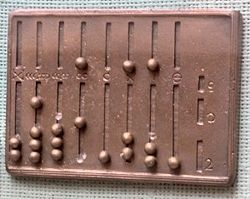
\includegraphics[scale=0.5]{img/Roman-abacus}
 \caption{现代复原的罗马算盘,在盘上开槽,槽中摆放石子,槽上标有罗马数字单位I, V, X, C, M。}
 \label{fig:roman-abacus}
 %https://www.newworldencyclopedia.org/entry/Abacus
\end{figure}

印度-阿拉伯计数系统传入欧洲后,尽管计算方便,人们还是把计算结果转换成罗马数字,而避免使用零\footnote{古代中国在进行算筹计算时(见第\ref{counting-rods}节)用空位代表0。但计算完成后就把结果用乘法分组系统表示出来,如一百、两千一十五、一百有二。汉字“零”直到宋、元后才出现。}。教会宣布0是邪恶的符号,禁止在公开场合使用。僧侣学者们用算盘(如\cref{fig:roman-abacus},不是中国明代发明的珠算)计算。欧洲的算盘源自古巴比伦的泥板。就是在一块板上用小石子按照罗马数字演算,算好后抄下结果。但商人们、银行家们看到了印度-阿拉伯数字的巨大好处,于是产生了十六世纪的“人机大战”,如\cref{fig:hindu-arabic-vs-abacus}。结果可想而知。自然是代表印度——阿拉伯计数的“机”胜了。这种“人机大战”在历史上一再上演:斯蒂芬森的火箭号列车\footnote{英国工程师乔治·斯提芬森和其子罗伯特·斯蒂芬森于1830年设计制造的蒸汽机车。}和马赛跑;深蓝挑战国际象棋大师卡斯帕罗夫;Alpha-Go挑战九段棋手李世石、柯洁;ChatGPT挑战大学生入学考试……每当有新事物出现,就有精彩的人机大战。

\begin{figure}[htbp]
 \centering
 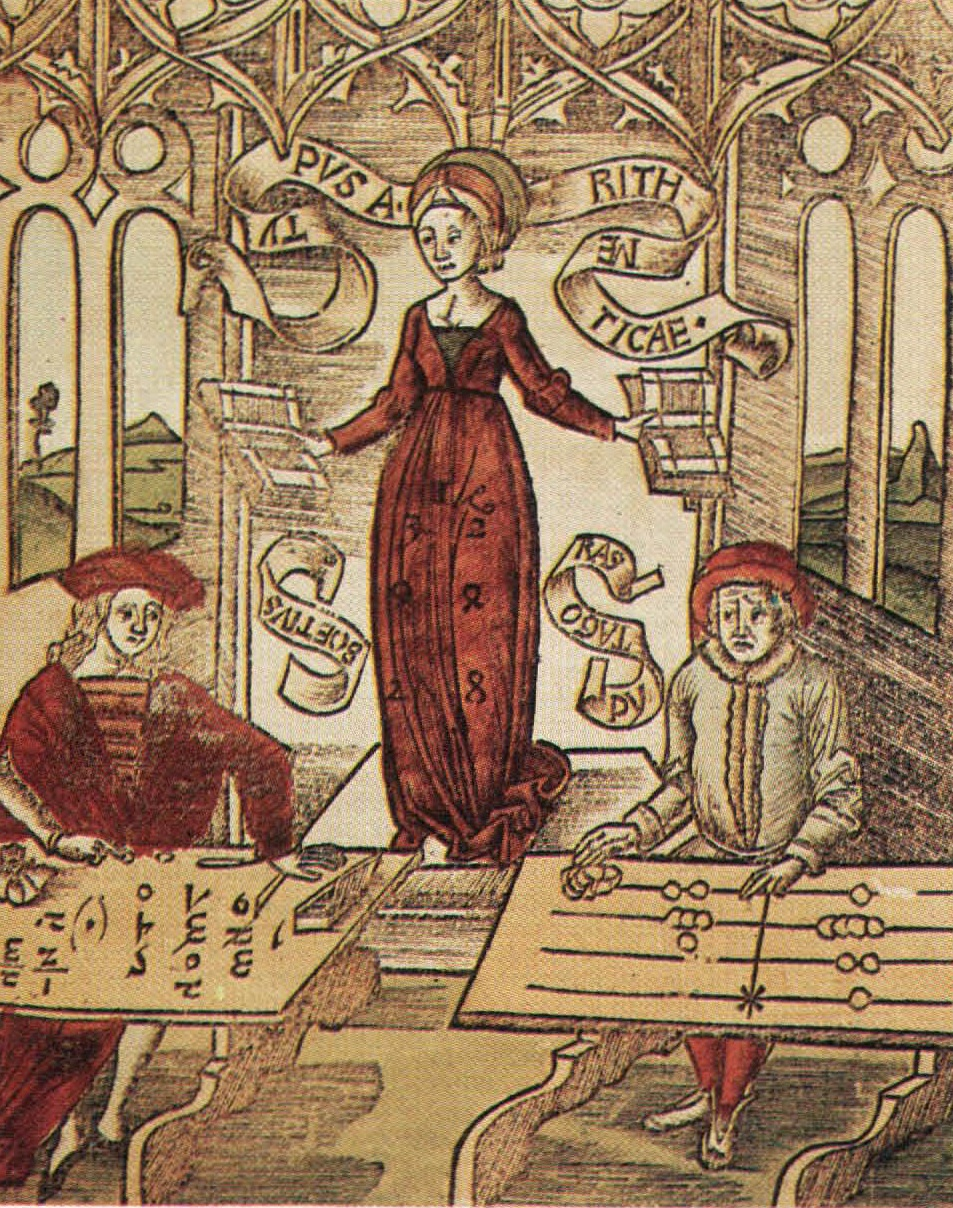
\includegraphics[scale=0.8]{img/Hindu-arabic-vs-abacus}
 \caption{1503年的版画。描绘了一个人用印度——阿拉伯数字计算,另一个人用罗马算盘计算的比赛。}
 \label{fig:hindu-arabic-vs-abacus}
 %https://www.newworldencyclopedia.org/entry/Abacus
\end{figure}

“机”的胜利让0具有了“二等公民”的身份——可以被使用了。可是为何0不能像1、2、3……那样成为“一等公民”呢?

\section{真正的数}

要想成为一等公民,0和1、2、3……比差了什么呢?是值,或者说大小。1这个符号代表的大小是1,比如1厘米的长度、1克的质量、1只羊……同样,2的值可以代表2厘米的长度、2克质量、2只羊……可是0呢?它没有值。“0是个占位符,不是一个数,因为它没有值\cite{Seife-2000}。”0极特殊,它表现得像一个破坏者,而非1、2、3……那样的“良民”。我们看看0是如何“破坏规矩”的:

\begin{enumerate}[(1)]
\item 阿基米德公理
\begin{align*}
1 + 1 &= 2   & 1 + 1 + 1 &= 3 & \dots \\
1 + 1 &= 2   & 1 + 1 + 1 &= 3 & \dots \\
1 + 1 &= 2   & 1 + 1 + 1 &= 3 & \dots \\
\dots &      & \dots     &    &
\end{align*}
一个数\footnote{本节的数都是自然数。}加上自己越来越大。阿基米德甚至指出这个规律是一个公理,今天叫做阿基米德公理:任意非零的$m < n$,则反复$m + m + \cdots$将会超过$n$。但 0 + 0 = 0没有变大,$0 + 0 + 0 + \cdots$不会超过任何数,包括1。

\item 积与面积

各个文明在丈量土地时都独立发展出了面积的概念,并将面积和乘法联系了起来。一块长方形的土地面积就是长与宽的积。$1 \times 5 = 5$代表宽1长5的矩形面积;$2 \times 5 = 10$代表宽2长5的矩形面积;$3 \times 5 = 15$代表宽3长5的矩形面积是……但是$0 \times 5$呢?矩形不见了,“坍缩”成了一个点\footnote{按欧几里得的定义,线段是没有宽度的,为什么矩形不是退化成了一条长5的线段?如果我们考虑长度的单位,例如厘米,则面积的单位是平方厘米。$0 \times 5 = 0$平方厘米,而线段只有长度,单位是5厘米。0平方厘米 $\neq$ 5厘米。},如图\cref{fig:rectangle-vanish},矩形消失了。

\begin{figure}[htbp]
 \centering
 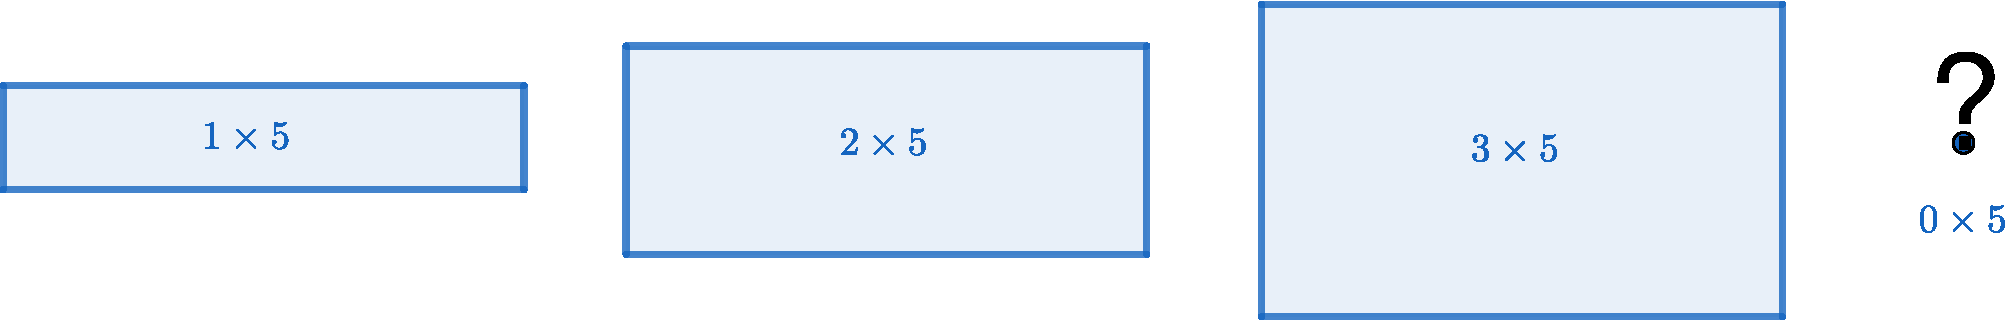
\includegraphics[scale=0.6]{img/rectangles}
 \caption{$0 \times 5$把矩形“压缩”成了一个没有大小的点。}
 \label{fig:rectangle-vanish}
\end{figure}

乘法还表示缩放。把一把尺子放大2倍,不仅尺子长度乘以2,尺子上的刻度间隔也乘以2;同样把尺子放大3倍,尺子的长度乘以3,刻度间隔也乘以3,如\cref{fig:ruler-vanish}。相反,把图中最大的尺子缩小3倍,即乘以$\frac{1}{3}$,则得到图中最小的尺子。但是如果缩放0倍,乘以0,整条尺子连同上面的刻度都“坍缩”成一点。尺子消失了。

\begin{figure}[htbp]
 \centering
 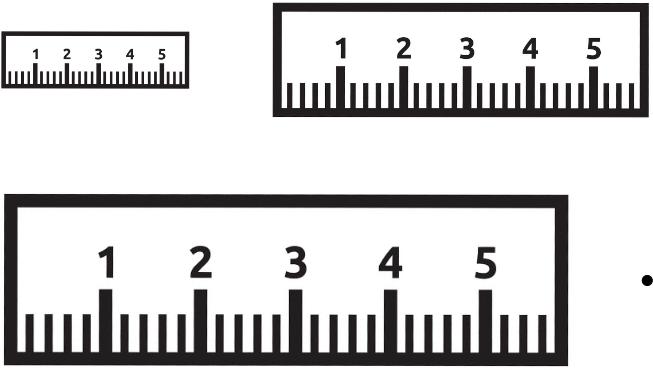
\includegraphics[scale=0.35]{img/zoom-rulers}
 \caption{缩放0倍把尺子连同刻度都“压缩”成了一个没有大小的点。}
 \label{fig:ruler-vanish}
\end{figure}

尺子代表了线段,乘以0破坏了矩形和线段。在古希腊发展几何学的时候还没有零的概念。古希腊的计数系统中也没有零。欧几里得定义“\textbf{点}是没有部分的”,“\textbf{线}只有长度而没有宽度”\footnote{欧几里得《几何原本》定义1、2。}。0对应几何学中的一个点么?

\item 乘除法的可逆性

除法被定义为乘法的逆运算。既然$2 \times 3 = 6$则$6 \div 2 = 3$;既然$3 \times 4 = 12$则$12 \div 3 = 4$……据此$2 \times 0 = 0$则$0 \div 2 = 0$,并且$a \times 0 = 0$故$0 \div a = 0$。但是0可以作除数么?根据逆运算,除法$a \div b$相当于求$c$使得$bc = a$,则$a \div 0$相当于求一个数$x$使得$0x = a$。但$0x = 0$,若$a \ne 0$,则不存在任何数$x$满足这个要求,因为:$0x = 0 \ne a$;若$a = 0$,虽然$0 \times 0 = 0$,看似$0 \div 0 = 0$;但$1 \times 0 = 0$,这样$0 \div 0 = 1$看似也可以;同样$2 \times 0 = 0$,故似乎$0 \div 0 = 2$……既然任何$a \times 0 = 0$则$0 \div 0 = a$,即$0 \div 0$等于任何值。但这意味着$(0 \div 0) = 0 = 1 = 2 = 3 = \cdots$,代表“无”的0,等于代表“有”的1、2、3……无即是有,空即是色。逻辑学家罗素指出从一个假命题可以推出任何命题。如果$0 = 1$,我们可以推出$1 + 1 = 3$:

\begin{align*}
0 = 1 & \Rightarrow 1 = 2     & \text{两边} + 1 \\
      & \Rightarrow 1 + 1 = 3 & \text{把} 1 = 1 \text{加到两边}
\end{align*}

伊恩·斯图尔特给出了这样一个荒唐的例子\cite{Stewart-2019}:

一只猫有一只尾巴;

没有猫有八只尾巴。

把这两句话加起来:一只猫有九只尾巴。
\end{enumerate}

鉴于0的这些奇特的“破坏”性质,人们把0归为1、2、3……之外的异类,如\cref{fig:keyboard}所示,0被放到了1到9的后面。

\begin{figure}[htbp]
 \centering
 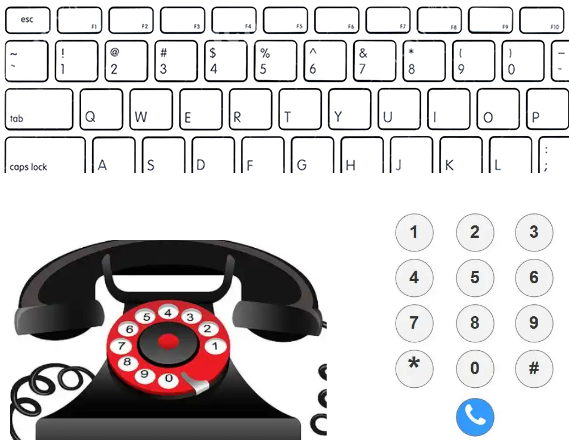
\includegraphics[scale=0.35]{img/keyboard}
 \caption{0在键盘上的位置}
 \label{fig:keyboard}
\end{figure}

\subsection{序数}

\ifx\wholebook\relax \else
\section{参考答案}
\shipoutAnswer


\begin{thebibliography}{99}

\bibitem{Seife-2000}
Charles Seife. ``Zero: the biography of a number'' Penguin Books, 2000. ISBN: 9-781-1011-9960-2

\bibitem{Stewart-2019}
[英]伊恩·斯图尔特 著,何生 译. ``不可思议的数'' 人民邮电出版社. 2019. ISBN: 978-7-115-51051-8

\end{thebibliography}

\expandafter\enddocument
\fi
